\documentclass[11pt,a4paper]{report}
\usepackage{geometry}
\usepackage{latexsym}
\usepackage{graphicx}
\usepackage{amsmath}
\usepackage[spanish]{babel}
\usepackage{multirow}
\usepackage{amssymb}
\usepackage{tikz}
\usepackage{subcaption}
\usepackage{natbib}

\newcommand*\circled[1]{\tikz[baseline=(char.base)]{
		\node[shape=circle,draw,inner sep=2pt] (char) {#1};}}
	

\setlength{\parindent}{0pt}

\date{}
\begin{document}
\title{Memoria Trabajo Lingüística Computacional}
\author{  Miguel Edo Goterris\and Roberto Labadie Tamayo}
	\date{Octubre 2022}
	\maketitle
	
	
	\section*{Tarea I}
		
		Para evaluar la tarea de etiquetado morfosintágtico empleando un HMM entrenado sobre el corpus \textbf{cess-esp} se estudian dos variantes, una sobre el conjunto de categorias original y otra con un conjunto de categorias reducidadas, que abarcan más palabras.\\
		
		A través de una validación cruzada con 10 particiones del dataset se obtienen los resultados mostrados en la \figurename~\ref{HMM_task1}.
		
		\begin{figure}[!thb]
		\begin{center}
			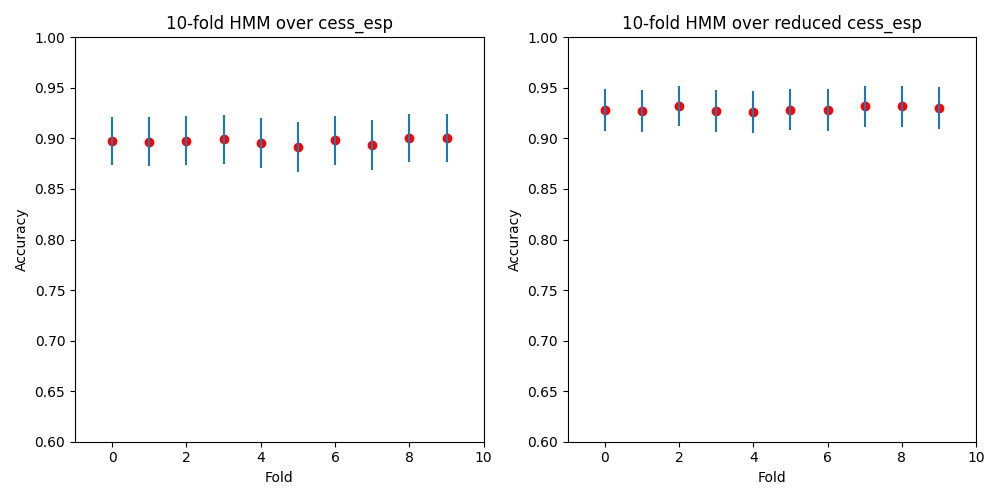
\includegraphics[scale=0.6]{images/HMM_task1.png}
		\end{center}
		\caption{Hidden Markov Model sobre cess-esp (izquierda) y cess-esp reducido (derecha) }
		\label{HMM_task1}
	\end{figure}
	
	Como se puede apreciar el desempeño del modelo con el dataset reducido es mejor debido a que la cantidad de estados ocultos del modelo es menor, por tanto la posibilidad de escoger una transición errada disminuye. Los tiempos de entrenamiento para el dataset reducido (9.27s) son menores que los del dataset original (33.77s). Esto se debe a que la complejidad del modelo es menor. En la gráfica se han incluido los intervalos de confianza. Nótese  que en ambos modelos la $i-esima$ partición es exactamente la misma, i.e., el mismo conjunto de elementos ordenados en ambos modelos. En el \tablename~\ref{HMM_task1_table} se muestran de manera detallada los resultados para cada variante.
	\begin{table}[thb!]
		\begin{center} 		
			\begin{tabular}{cc} 
				\hline	
				\multirow{2}{*}{\textbf{cess-esp}}&\textbf{reduced}\\
				&\textbf{cess-esp}\\
				\hline
				0.897$\pm$0.02&0.928$\pm$0.02\\
				0.897$\pm$0.02&0.927$\pm$0.02\\
				0.898$\pm$0.02&0.932$\pm$0.02\\
				0.899$\pm$0.02&0.928$\pm$0.02\\
				0.896$\pm$0.02&0.927$\pm$0.02\\
				0.892$\pm$0.02&0.928$\pm$0.02\\
				0.898$\pm$0.02&0.928$\pm$0.02\\
				0.893$\pm$0.02&0.932$\pm$0.02\\
				0.900$\pm$0.02&0.932$\pm$0.02\\
				0.900$\pm$0.02&0.930$\pm$0.02\\
				\hline
			\end{tabular}
			\caption{Accuracy de los corpus originales y reducido.}	
			\label{HMM_task1_table}
		\end{center}
	\end{table}		 	
	\\\\\\\\\\\\\\\\

	
	Teniendo en cuenta que la medida de accuracy nos da un valor suavizado del desempeño global de todas las etiquetas, analizamos la media de Macro-F1 para cada partición como se muestra en la \figurename~\ref{macro-f1-hmm}.
	
	\begin{figure}[!thb]
		\begin{center}
			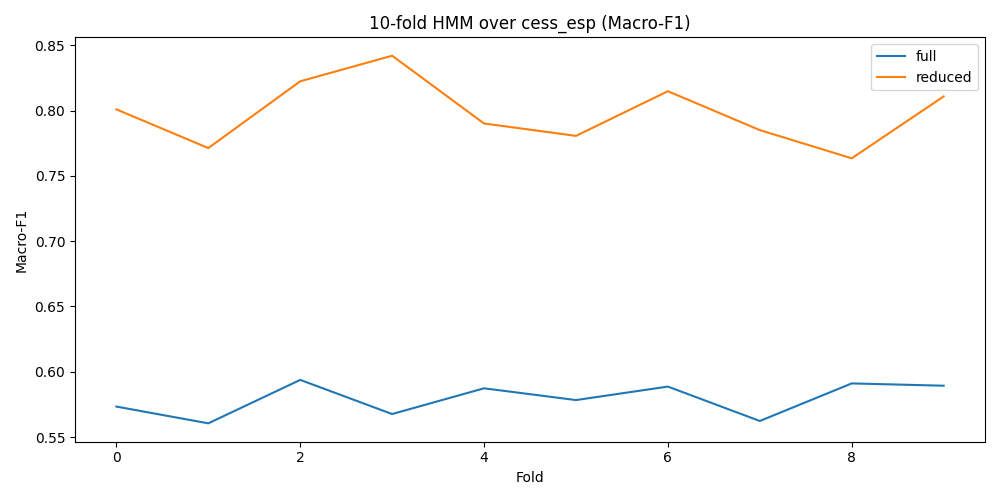
\includegraphics[scale=0.6]{images/macro-f1-hmm.png}
		\end{center}
		\caption{Macro-F1 Hidden Markov Model sobre cess-esp y cess-esp reducido}
		\label{macro-f1-hmm}
	\end{figure}

	De aquí podemos concluir que evidentemente hay etiquetas que están siendo mal predichas por el modelo, sobretodo para la tarea ampliada, lo que puede estar relacionado con una subrepresentación de estos fenómenos en el training-set. Teniendo en cuenta esto, resulta más coherente asumir un etiquetado más global y suavizado que permita tener para cada categoría más ejemplos de entrenamiento como el propuesto en la tarea reducida. En lo adelante emplearemos el conjunto de datos reducidos para evaluar los modelos.
	
	\section*{Tarea II}
	
	Despues de barajar el dataset para la tarea reducida y tomar los últimos $\Big\lceil \frac{|\mathcal{D}|}{10}\Big\rceil$ elementos para validar nuestro modelo, se observa una relación proporcional con el acuraccy y la cantidad de datos empleados para entrenamiento como se muestra en la \figurename~\ref{incremental-set}.
		
		
		\begin{figure}[!thb]
			\begin{center}
				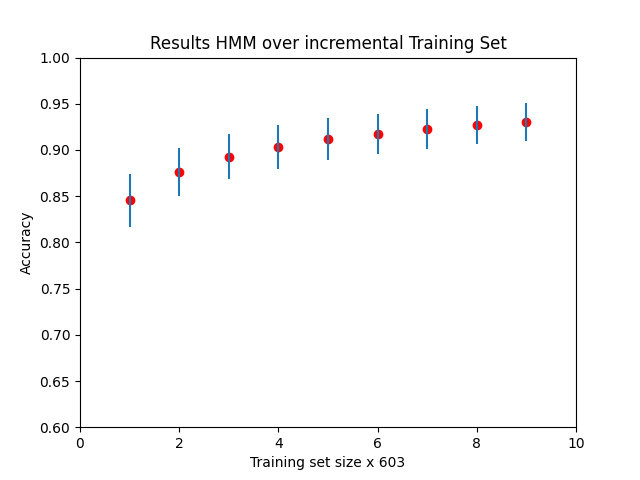
\includegraphics[scale=0.6]{images/incremental-set.png}
			\end{center}
			\caption{Accuracy Hidden Markov Model sobre cess-esp reducido y con incremento progresivo del conjunto de entrenamiento}
			\label{incremental-set}
		\end{figure}
		


	Efectivamente alcanzando el mejor desempeño para el conjunto de entrenamiento completo. Al igual que en la tarea anterior cuando empleamos el dataset ampliado y algunas etiquetas resultaban subrepresentadas, es posible concluir que en este caso sucede lo mismo para subconjuntos pequeños del dataset. Por otro lado dentro de un modelo estadístico como lo es el HMM, el número de observaciones de un suceso esta directamente relacionado con cuan preciso es el valor de probabilidad de ocurrencia calculado para este.\\
	
    	\begin{table}[thb!]
    		\begin{center} 		
    			\begin{tabular}{ccc} 
    				\hline	
    				\textbf{Tamaño corpus}&\textbf{Accuracy}&\textbf{Tiempo (s)}\\
    				\hline
                    603&0.782$\pm$0.032&17.617\\
                    1206&0.823$\pm$0.030&21.563\\
                    1809&0.845$\pm$0.028&25.071\\
                    2412&0.861$\pm$0.027&27.143\\
                    3015&0.869$\pm$0.026&28.519\\
                    3618&0.878$\pm$0.026&30.998\\
                    4221&0.884$\pm$0.025&31.490\\
                    4824&0.889$\pm$0.025&32.505\\
                    5427&0.893$\pm$0.024&33.393\\
    				\hline
    			\end{tabular}
    			\caption{Resultados dataset reducido variando el tamaño de corpus.}	
    			\label{HMM_task2_table}
    		\end{center}
    	\end{table}
	
	En el \tablename~\ref{HMM_task2_table} podemos ver como el tiempo tambien crece a medida que lo hace el corpus de entrenamiento.
	

	
	\section*{Tarea III}
	
	Para incorporar al Tnt el método de suavizado para palabras desconocidas mediante el uso de sufijos, primero estudiamos el comportamiento del método Affix Tagger  con varias longitudes de sufijos en el rango de 1 a 9 caracteres, en la ~\figurename~\ref{affix} se muestra el valor medio del accuracy para este método en un cross-validation que involucra el mismo conjunto de datos ordenados en cada fold para cada variante de sufijo.
	\vspace{-3mm}
	\begin{figure}[!thb]
		\begin{center}
			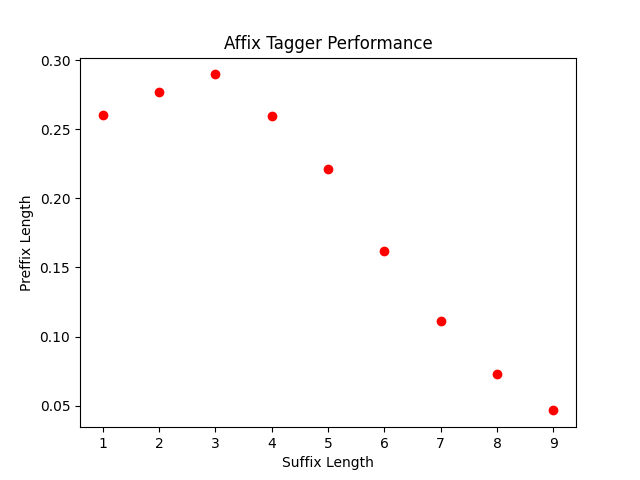
\includegraphics[scale=0.55]{images/affix.png}
		\end{center}
		\caption{ Accuracy Medio del método Affix Tagger sobre cross-validation en cess-esp reducido.}
		\label{affix}
	\end{figure}
	\vspace{-2mm}
	\\
	del anterior experimento, tomamos como longitud de sufijos para estudiar el suavizado en el Tnt $l=3$. En la \figurename~\ref{tnt-suffix} se muestran los resultados de introducir el suavizado.
		\begin{figure}[!thb]
		\begin{center}
			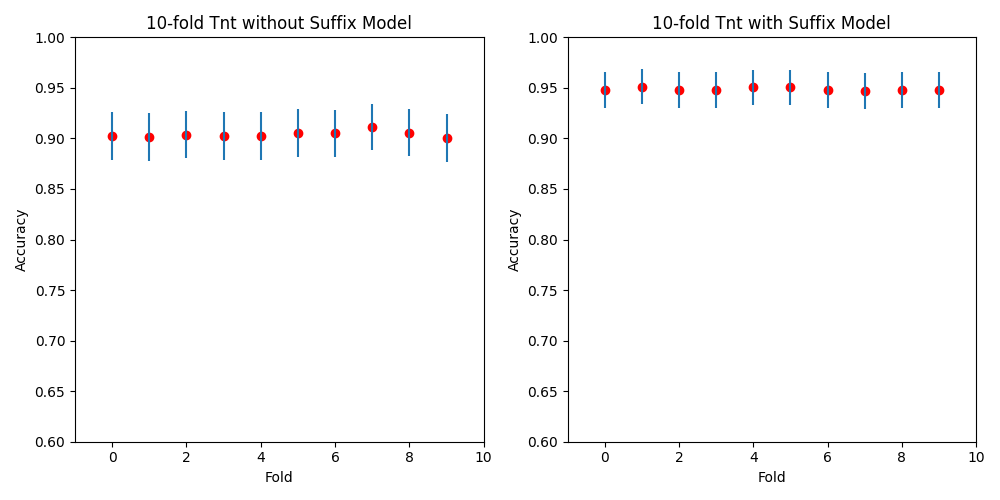
\includegraphics[scale=0.6]{images/tnt-suffix.png}
		\end{center}
		\caption{ Tnt Tagger vs Tnt Tagger con suavizado para palabras desconocidas.}
		\label{tnt-suffix}
	\end{figure}
	\\ 
	El desempeño del modelo incrementa en $\sim$5\% gracias a la inclusión de palabras no vistas en el conjunto de entrenamiento dentro categorías que parecen relacionarse con las mismas atendiendo a su sufijo, en el \tablename~\ref{tnt-comparison} se muestran los resultados de manera mas detallada.\\
	
			\begin{table}[thb!]
		\begin{center} 		
			\begin{tabular}{cc} 
				\hline	
				\textbf{Tnt+suffix}&\multirow{2}{*}{\textbf{Tnt}}\\
				\textbf{smoth}&\\
				\hline
				0.948$\pm$0.018&0.903$\pm$0.024\\
				0.951$\pm$0.017&0.901$\pm$0.024\\
				0.948$\pm$0.018&0.904$\pm$0.024\\
				0.948$\pm$0.018&0.903$\pm$0.024\\
				0.950$\pm$0.017&0.902$\pm$0.024\\
				0.950$\pm$0.017&0.905$\pm$0.023\\
				0.948$\pm$0.018&0.905$\pm$0.023\\
				0.947$\pm$0.018&0.911$\pm$0.023\\
				0.948$\pm$0.018&0.906$\pm$0.023\\
				0.948$\pm$0.018&0.900$\pm$0.024\\
				\hline
			\end{tabular}
			\caption{Valores de Acuraccy con respectivos intervalos de confianza para cross-validation Tnt y Tnt suavizado para palabras no vistas.}	
			\label{tnt-comparison}
		\end{center}
	\end{table}		 	
	El tiempo no varia de forma significativa, pasando de 94.63 segundos por iteracion sin Affix tagger a 95.52 s/it con este. 
	

	\section*{Tarea IV}

    Para esta tarea se han usado multiples paradigmas de etiquetado. Para cada uno se ha calculado su accuracy con su respectivo intervalo de confianza. Los resultados se pueden ver en el \tablename~\ref{table-task4}. Como se puede apreciar el paradigma que ha dado peores resultados es el de unigramas. Esto era de esperar puesto que es el más simple y el que ofrece una menor reducción de la entropia. Acto seguido, con una sensible mejora esta el de bigramas. A continuación podemos observar un conjunto de paradigmas que han generado resultados similares, el paradigma de Brill con unigramas o bigramas y distintos numeros de reglas maximas. Estos metodos siguien siendo bastante simples y un incremento en el numero de reglas no introduce una mejora puesto que las normas más relevantes y que contribuyen a una mayor reduccion de la entropia estan presentes en el primer grupo de 256 reglas. A continuación estan los conocidos paradigmas tnt y hmm. Como ya descubrimos en la practica 2 el hmm funciona bastante mejor que el tnt. La combinación de Brill y hmm introduce una ligera pero importante mejora. Por ultimo, el modelo basado en el perceptron tiene una accuracy muy superior al resto.\\
    
    Si nos fijamos en los tiempos podemos ver como el accuracy no tiene una relacio directa con el tiempo de entrenamiento. Hay modelos muy lentos que generan resultados mediocres, como brill-unigram, y otros muy rapidos con estupendos resultados, como el perceptron. 

		\begin{table}[thb!]
		\begin{center} 		
			\begin{tabular}{cc} 
				\hline	
				\textbf{Paradigma}&\textbf{Accuracy}\\
				\hline
                unigram&0.883$\pm$0.026\\
                tagger-bigram&0.900$\pm$0.024\\
                brill-unigram-256&0.905$\pm$0.023\\
                brill-bigram-256&0.905$\pm$0.023\\
                brill-unigram-512&0.906$\pm$0.023\\
                brill-bigram-512&0.905$\pm$0.023\\
                brill-unigram-1024&0.906$\pm$0.023\\
                brill-bigram-1024&0.905$\pm$0.023\\
                Tnt&0.906$\pm$0.023\\
                HMM&0.928$\pm$0.021\\
                brill-hmm-256&0.931$\pm$0.020\\
                brill-hmm-512&0.931$\pm$0.020\\
                brill-hmm-1024&0.931$\pm$0.020\\
                perceptron-tagger&0.963$\pm$0.015\\
				\hline
			\end{tabular}
			\caption{Distintos paradigmas de etiquetado con el accuracy obtenido.}	
			\label{table-task4}
		\end{center}
	\end{table}		 
	
			\begin{table}[thb!]
		\begin{center} 		
			\begin{tabular}{ccc} 
				\hline	
				\textbf{Paradigma}&\textbf{Accuracy}&\textbf{Tiempo}\\
				\hline
	            unigram&0.879$\pm$0.026&0.033\\
                bigram&0.895$\pm$0.024&0.054\\
                brill-unigram-256&0.899$\pm$0.024&28.875\\
                brill-bigram-256&0.900$\pm$0.024&12.157\\
                brill-unigram-512&0.900$\pm$0.024&40.447\\
                brill-bigram-512&0.900$\pm$0.024&12.502\\
                brill-unigram-1024&0.900$\pm$0.024&41.025\\
                brill-bigram-1024&0.900$\pm$0.024&11.838\\
                Tnt&0.901$\pm$0.024&70.561\\
                HMM&0.930$\pm$0.020&8.750\\
                brill-hmm-256&0.934$\pm$0.020&82.122\\
                brill-hmm-512&0.934$\pm$0.020&93.509\\
                brill-hmm-1024&0.934$\pm$0.020&94.086\\
                perceptron-tagger&0.988$\pm$0.009&1.074\\
				\hline
			\end{tabular}
			\caption{Distintos paradigmas de etiquetado con el accuracy obtenido.}	
			\label{table-task4}
		\end{center}
	\end{table}		
	
	\section*{Tarea V}
	La primera herramienta que analizaremos es FreeLing. De los tres proyectos sugeridos este parece ser el más pequeño. Es opensource y la ultima actualización de su repositorio es de hace aproximadamente 3 meses, es decir, se mantiene actualizado. Ofrece un conjunto de funcionalidades que cubre las necesidades básicas como POS-tagging, parsing, wsd, named entity detection etc. Soporta 14 idiomas. Dado que es un proyecto que surge en España entre estos idiomas podemos encontrar el español, catalan, gallego y asturiano. Contiene diccionarios para todos estos idiomas, obtenidos de distintos proyectos opensource y información semantica para el ingles, catalan, español, gallego, italiano, portgues, esloveno y croata.. La documentación parece ser bastante completa, los conceptos se explican con suficiente claridad y la API de c++ esta comentada, aunque no ofrece una guia de iniciacion del tipo "get started" que siempre es de gran utilidad.  El proyecto esta desarrollado en C++ y se puede interactuar con el mediante la linea de comandos o bindings para java o python. Para nosotros es de interes los bindings de python. Existen binarios para una facil instalación en windows, aunque en la guia oficial indica que se hace compilar el codigo fuente para hacer uso de los bindings de python. Es necesario instalar manualmente las dependencias y usar cmake para compilar el proyecto. En base a mi experiencia no tengo ninguna esperanza de que, pese a que se sigan las instrucciones al pie de la letra, funcione a la primera. Descartaria esta herramienta solo por su dificultad de instalación. Como veremos en las otras herramientas este paso es tremendamente mas facil.\\
	
	Stanza parece ser un proyecto mucho mas establecido que FreeLing. Tambien es opensource y su ultima actualización es de hace aproximadamente un mes. Tambien es capaz de llevar a cabo todas las funciones que podamos necesitar y Tiene modelos preentrenados de mas de 70 idiomas . Esta implementado en python puro usando pythorch y hace un uso extensivo de las redes neuronales, por lo que puede ser acelerado por GPU. Esta bien documentado, con ejemplos en python y tiene una guia de inicio rapido. Su instalación es muy simple, como cabria esperar de un paquete de python. No es necesario ninguna configuracion y con unas pocas lineas podemos llevar a cabo el analisis morfosintactico:\\
	
	\begin{verbatim}
!pip install stanza
import stanza
nlp = stanza.Pipeline('es')
with open('/content/Alicia_utf8.txt', 'r') as file:
    doc = nlp(file.read())
    for sentence in doc.sentences:
        for word in sentence.words:
            print(word.text, word.pos)
    \end{verbatim}
    
    Por ultimo tenemos SpaCy. SopaCy tambien es opensource y su ultima actualización es de hace 4 dias. Si miramos sus metricas en github podemos ver que claramente es el mas popular de las tres opciones con diferencia. Por lo demas, para el uso que nosotros le podriamos dar, es bastante similar a Stanza. Esta programado con python, tiene todas las caracteristicas que podamos necesitar, se un uso extensivo de redes neuronales, cubre una cantidad de lenguajes muy extensa con modelos preentrenados, es facil de instalar y de usar, tiene buena documentación y una guia de inicio rapido. Parece estar más orientado a la producción, lo cual depende del uso que se le vaya dar puede ser interesante. Tiene una seccion de benchmarks en los cuales podemos observar que tiene una precisión que lo posiciona en el state of the art y la cantidad de palabras que puede procesar por segundo es muy superior a las alternativas (entre ellas Stanza). A continuación el codigo necesario para analizar morfosintacticamente un texto:
    
    	\begin{verbatim}
!pip install spacy
!pip install es-core-news-sm
import spacy
nlp = spacy.load("es_core_news_sm")
with open('/content/Alicia_utf8.txt', 'r') as file:
    data = file.read()
    doc = nlp(data)
    for token in doc:
        print(token.text, token.pos_)
    \end{verbatim}
    
    A falta de un analisis en mayor profundidad consideraria tanto Stanza como SpaCy dos opciones muy validas. Trataria de apartarme de FreeLing por su dificultad de instalación y documentación escueta si la comparamos con las otras dos opciones. Tanto SpaCy como Stanza se pueden ejecutar desde google colaboratory sin ninguna dificultad, lo cual facilita su uso en el aula y la colaboración entre compañeros. Personalmente me decantaria por SpaCy porque cumple sobradamente con nuestras necesidades y ademas tiene una comunidad mucho más grande que Stanza, lo cual significa que hay más tutoriales, más documentación, más potenciales problemas solucionados etc. Ademas es una herramienta que a parte de interesante para el aprendizaje tambien lo es para el desarrollo de proyectos serios. Stanza tarda 4.93s en hacer Pos-tagging delfichero Alicia.txt mientras que SpaCy tan solo tarda 0.436, unas 11 veces más rápido.
    
	\section*{Preguntas}
	
	\textbf{Es interesante usa brill para bigramas y unigramas? y para hmm?}\\
	No. Sí.\\
	
	
	\textbf{Srería interesante incrementar el tamaño del training set?}\\
	Sí, puesto que aunqe la mejora es pequeña el incremento temporal es muy bajo, sobre todo si usamos paradigmas rapidos como Hmm o perceptron.
    	
    	

\end{document}